\section{Esercizio 3 -- Riconoscitore di sequenze}
\subsection{Esercizio 3.1}
L'architettura del riconoscitore di sequenze è stata progettata per identificare la sequenza binaria ``101", sia in modalità non sovrapposta che parzialmente sovrapposta. La FSM è composta da sette stati. All'arrivo di \texttt{M}, la variabile \texttt{current\_mode} passa da 0 a 1 o viceversa e la macchina ritorna in $S_0$ [Figura \ref{fig:sequence_detector}].

\begin{figure}[h]
    \centering
    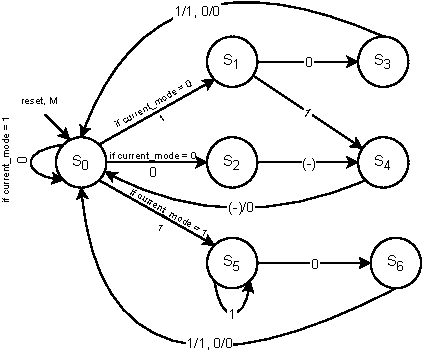
\includegraphics[width=0.55\linewidth]{img/sequence_detector.pdf}
    \caption{Automa del riconoscitore di sequenze}
    \label{fig:sequence_detector}
\end{figure}

\subsubsection{Implementazione}
\begin{code}
    \inputminted{vhdl}{vhdl/Sequence_Detector.vhd}
    \caption{Implementazione del riconoscitore di sequenze}
    \label{cod:sequence_detector}
\end{code}

L'entity è la parte del codice che descrive i segnali di ingresso e uscita del modulo:

\begin{itemize}
    \item \texttt{input}: bit da analizzare.
    \item \texttt{M}: segnale che seleziona la modalità operativa della FSM.
    \item \texttt{reset}: riporta la FSM allo stato iniziale.
    \item \texttt{clock}: sincronizza la FSM con il segnale di clock.
    \item \texttt{A}: abilita la FSM.
    \item \texttt{state\_output\_led}: uscita a 7 bit per rappresentare lo stato corrente sui LED.
    \item \texttt{Y}: uscita che si attiva quando viene riconosciuta la sequenza.
\end{itemize}

L'architettura, che è \texttt{behavioral} [Codice sorgente \ref{cod:sequence_detector}], è la parte in cui avviene la dichiarazione della FSM:

\begin{itemize}
    \item \texttt{current\_mode} memorizza la modalità attuale (M).
    \item \texttt{stato} definisce i sette stati della macchina (S0--S6).
    \item \texttt{current\_state} tiene traccia dello stato attuale.
    \item \texttt{fsm\_encoding} specifica la codifica degli stati in formato one-hot, dove ogni stato è rappresentato da un solo bit attivo alla volta.
\end{itemize}

A questo punto, si definisce il processo principale, attivo sul fronte di salita del clock, garantendo che la FSM sia sincronizzata con il sistema.

\begin{itemize}
    \item Se il reset è attivo (\texttt{reset = `1'}) o la modalità cambia (\texttt{M} cambia rispetto al valore precedente), la FSM ritorna allo stato iniziale $S_0$.
    \begin{itemize}
        \item L'uscita \texttt{Y} viene azzerata (\texttt{Y <= `0'}).
        \item Viene aggiornato il valore di \texttt{current\_mode}.
    \end{itemize}
    \item Altrimenti, se il segnale di abilitazione \texttt{A} è attivo, la FSM può elaborare i dati (si utilizza un \texttt{case} per gestire la transizione tra gli stati).
    \begin{enumerate}
        \item Nello stato $S_0$, l'uscita \texttt{Y} viene azzerata nel caso sia stata attivata in cicli precedenti. A seconda della modalità (\texttt{M}), la FSM segue due percorsi diversi:
        \begin{enumerate}
            \item Se \texttt{M = 0}:
            \begin{enumerate}
                \item \texttt{input = 0} $\rightarrow$ passa a $S_2$.
                \item \texttt{input = 1} $\rightarrow$ passa a $S_1$.
            \end{enumerate}
            \item Se \texttt{M = 1}:
            \begin{enumerate}
                \item \texttt{input = 0} $\rightarrow$ rimane in $S_0$.
                \item \texttt{input = 1} $\rightarrow$ passa a $S_5$.
            \end{enumerate}
        \end{enumerate}
        \item $S_1$ e $S_2$ portano agli stati $S_3$ o $S_4$ in base all'input.
        \item In $S_3$, l'uscita \texttt{Y} prende il valore di input e si torna a $S_0$.
        \item In $S_4$, \texttt{Y} è 0 e si torna a $S_0$.
        \item $S_5$ è il primo stato per \texttt{M = 1} e porta a $S_6$ quando \texttt{input = 0}.
        \item $S_6$ attiva \texttt{Y} e torna a $S_0$.
    \end{enumerate}
\end{itemize}

\subsubsection{Simulazione}
Per effettuare la simulazione il primo passo da compiere è la stesura del testbench. Prima di discutere quanto fatto è bene osservare il codice in figura:

\begin{code}
    \inputminted{vhdl}{vhdl/Sequence_Detector_tb.vhd}
    \caption{Testbench del riconoscitore di sequenze}
    \label{cod:sequence_detector_tb}
\end{code}

La prima operazione svolta è stata la dichiarazione di un’entity. Si può notare che il corpo dell’entity è vuoto, poiché il testbench non rappresenta un componente hardware da implementare, ma serve esclusivamente per la simulazione e la verifica del corretto funzionamento del sistema.

Nell’architettura \texttt{behavioral} viene dichiarato il solo componente che sarà testato:

\begin{itemize}
    \item \texttt{Sequence\_Detector}: permette di instanziare il modulo all'interno del testbench.
\end{itemize}

Vengono dichiarati diversi segnali che serviranno per la simulazione:

\begin{enumerate}
    \item \texttt{CLK\_period}: definisce il periodo di clock a 10 ns.
    \item \texttt{input}: segnale di ingresso inizializzato a 0.
    \item \texttt{M}: modalità operativa della FSM inizializzata a 0.
    \item \texttt{reset}: segnale di reset inizialmente attivo (1).
    \item \texttt{clock}: segnale di clock inizialmente 0.
    \item \texttt{enable}: segnale di abilitazione della FSM inizialmente 0.
    \item \texttt{output}: uscita Y inizialmente 0.
\end{enumerate}

Dopo aver dichiarato il componente, avviene il port mapping e la generazione del clock:

\begin{itemize}
    \item Nel primo caso, creiamo un'istanza del modulo \texttt{Sequence\_Detector} e colleghiamo i segnali del testbench ai suoi ingressi e uscite.
    \item Nel secondo caso, il processo \texttt{CLK\_process} genera un segnale di clock con periodo di 10 ns, che oscilla tra 0 e 1 ogni 5 ns, ottenendo così una frequenza di 100 MHz.
\end{itemize}

Nel processo di simulazione \texttt{stim\_process}, dopo 100 ns, si abilita la FSM (\texttt{A = 1}) e disattiviamo il reset (\texttt{reset = 0}). A questo punto, il Sequence Detector è pronto per ricevere gli ingressi, mandando prima la sequenza \texttt{000101}, che dovrebbe essere riconosciuta dalla FSM in modalità non sovrapposta, con un controllo in cui se \texttt{output} non è 1 al termine della sequenza, viene segnalato un errore e poi cambiando la modalità in parzialmente sovrapposta, inviando una nuova sequenza di bit. Anche in questo caso, se output non diventa 1, viene segnalato un errore [Figura \ref{fig:sequence_detector_tb}].

\begin{figure}[h]
    \centering
    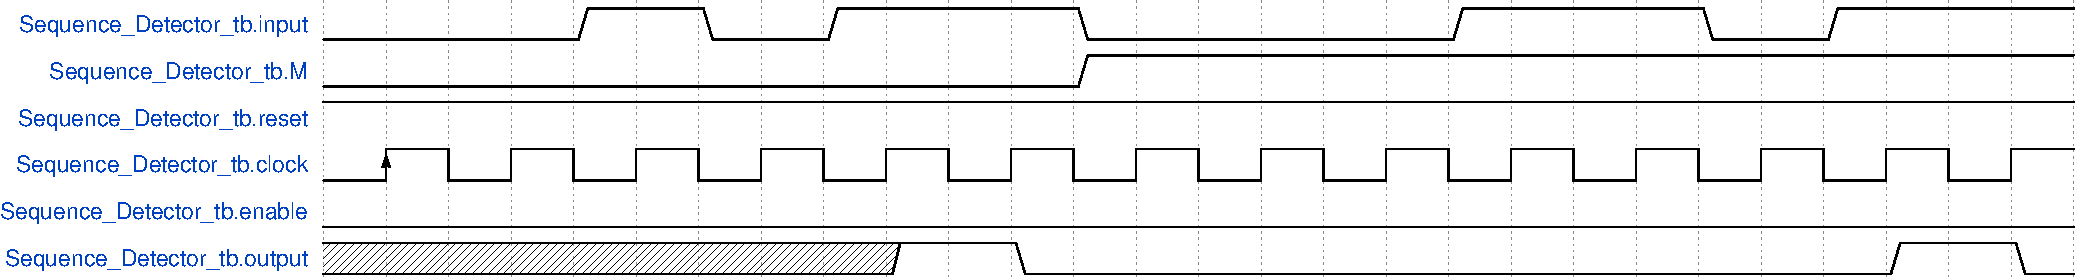
\includegraphics[width=\linewidth]{img/sequence_detector_tb.pdf}
    \caption{Simulazione del riconoscitore di sequenze}
    \label{fig:sequence_detector_tb}
\end{figure}

\subsection{Esercizio 3.2}
Si implementa un riconoscitore di sequenze su FPGA, utilizzando switch, pulsanti e LED per interagire con l'utente. Il riconoscitore è basato su un automa a stati finiti, che cambia stato in base agli ingressi forniti e accende un LED quando una specifica sequenza viene riconosciuta.

\begin{code}
    \inputminted{vhdl}{vhdl/Sequence_Detector_onboard.vhd}
    \caption{Implementazione del riconoscitore di sequenze su board}
    \label{cod:sequence_detector_onboard}
\end{code}

\begin{code}
    \inputminted{vhdl}{vhdl/sequence_Detector_Input_Manager.vhd}
    \caption{Implementazione del gestore degli input}
    \label{cod:sequence_detector_input_manager}
\end{code}

\paragraph{Funzionamento generale.}
Il funzionamento del sistema è schematizzabile in cinque punti:

\begin{enumerate}
    \item Input dell'utente tramite switch e pulsanti.
    \begin{itemize}
        \item \texttt{S1} (\texttt{SW14}): codifica il bit di ingresso (\texttt{i}).
        \item \texttt{S2} (\texttt{SW15}): codifica la modalità (\texttt{M}).
        \item \texttt{B1} (\texttt{BTNL}): acquisisce il valore di \texttt{i} dallo switch \texttt{S1}.
        \item \texttt{B2} (\texttt{BTNR}): acquisisce la modalità \texttt{M} dallo switch \texttt{S2}.
    \end{itemize}
    \item Gestione del segnale di temporizzazione.
    \begin{itemize}
        \item Viene generato un segnale \texttt{A}, a partire dal clock della scheda.
        \item \texttt{A} viene usato per sincronizzare il riconoscitore.
    \end{itemize}
    \item Elaborazione della sequenza.
    \begin{itemize}
        \item Il riconoscitore aggiorna il suo stato basandosi su \texttt{i}, \texttt{M} e \texttt{A}.
        \item I sette LED di destra mostrano lo stato attuale dell'automa.
    \end{itemize}
    \item Indicazione del riconoscimento.
    \begin{itemize}
        \item Quando la sequenza è riconosciuta, il primo LED di sinistra si accende.
        \item Se la modalità \texttt{M} cambia, il sistema viene resettato automaticamente.
    \end{itemize}
    \item Reset del sistema.
    \begin{itemize}
        \item Il pulsante superiore (\texttt{BTNU}) riporta il riconoscitore allo stato iniziale.
    \end{itemize}
\end{enumerate}

\paragraph{Struttura del codice.}
L’architettura è \texttt{structural} [Codice sorgente \ref{cod:sequence_detector_onboard}], ovvero il sistema è composto da diversi moduli interconnessi:

\begin{enumerate}
    \item \texttt{Sequence\_Detector\_onboard}: definisce gli ingressi e le uscite del sistema.
    \begin{itemize}
        \item \texttt{CLK100MHZ}: clock della FPGA.
        \item \texttt{SW(15)}: \texttt{S2}, switch per selezionare la modalità \texttt{M}.
        \item \texttt{SW(14)}: \texttt{S1}, switch per impostare il valore dell'input \texttt{i}.
        \item \texttt{BTNL}: pulsante per acquisire \texttt{i}.
        \item \texttt{BTNR}: pulsante per acquisire \texttt{M}.
        \item \texttt{BTNU}: pulsante di reset.
        \item \texttt{LED\_STATE}: mostra lo stato dell'automa (7 LED).
        \item \texttt{LED\_OUTPUT}: indica quando la sequenza è riconosciuta.
    \end{itemize}
    \item \texttt{Sequence\_Detector}: gestisce l'automa.
    \begin{itemize}
        \item \texttt{state\_output\_led}: indica lo stato corrente con 7 LED.
        \item \texttt{Y}: si attiva quando la sequenza è riconosciuta.
    \end{itemize}
    \item \texttt{Input\_Manager}: interpreta i valori degli switch e dei pulsanti [Codice sorgente \ref{cod:sequence_detector_input_manager}].
    \begin{itemize}
        \item \texttt{load\_next}: acquisisce \texttt{i} quando \texttt{BTNL} viene premuto.
        \item \texttt{change\_mode}: acquisisce \texttt{M} quando \texttt{BTNR} viene premuto.
        \item \texttt{detector\_enable}: genera il segnale \texttt{A} di sincronizzazione.
    \end{itemize}
    \item \texttt{Button\_Debouncer}: stabilizza il segnale dei pulsanti, evitando falsi rilevamenti dovuti ai rimbalzi meccanici [Codice sorgente \ref{cod:button_debouncer}].
\end{enumerate}

\paragraph{Collegamento dei componenti.}
I moduli sopra indicati vengono collegati tra loro in modo da formare il sistema complessivo:
\begin{enumerate}
    \item \texttt{seq\_detector}: il riconoscitore analizza i segnali e aggiorna lo stato e il LED di uscita.
    \item \texttt{input\_mgr}: interpreta i valori degli switch e aggiorna i segnali \texttt{detector\_input} e \texttt{detector\_M}.
    \item \texttt{btn\_debouncer\_left}: filtra il segnale di \texttt{BTNL}, garantendo che l'input \texttt{i} sia acquisito correttamente.
    \item \texttt{btn\_debouncer\_right}: filtra il segnale di \texttt{BTNR}, garantendo che la modalità \texttt{M} sia acquisita correttamente.
\end{enumerate}

Per poter utilizzare la board è stato necessario effettuare alcune modifiche al file dei constraints \texttt{Nexys A7-100T-Master.xdc}. In particolare, abbiamo dovuto aggiungere i seguenti vincoli:
\begin{itemize}
    \item Abilitare il clock a 100 MHz.
    \item Abilitare gli switch \texttt{SW14} ed \texttt{SW15} per l’input.
    \item Abilitare i pulsanti \texttt{BTNL} e \texttt{BTNR} per il controllo del caricamento dei dati, \texttt{BTNU} per il reset.
    \item Abilitare i LED \texttt{LED0}--\texttt{LED6} per la visualizzazione dello stato, \texttt{LED15} per la visualizzazione dell’output.
\end{itemize}
